\documentclass[letterpaper]{article}

\newif\ifpresentation

\usepackage[margin=1in]{geometry}
\usepackage{amsmath}
\usepackage{graphicx}
\usepackage{hyperref}
\usepackage{booktabs}
\usepackage{xcolor}
\pagecolor{white}

\title{Correctness and Performance Analysis of Parallel Sorting Algorithms}
\author{Akshat Rohella \and Aaron Johnson \and Aditya Behre}
\date{April 2026}

\begin{document}
\maketitle

\section{Introduction}
As Rosca and C\u{a}rbureanu explain, sorting algorithms are essential in computer science, and they influence ``the efficiency of applications that operate on large-scale datasets,'' which is important as modern programs often handle large amounts of data \cite{rosca}.

The goal of this project is to explore how parallelism can improve the performance of sorting algorithms while still maintaining correctness. Specifically, we implemented both sequential and parallel versions of the quicksort and merge sort algorithms, and analyzed how their performance changes when multiple threads are used. Quicksort and merge sort are very popular algorithms with average-case time complexity $O(n \log n)$, and both follow a divide-and-conquer structure which makes them well suited for parallel execution. By implementing both sequential and parallel versions, we can directly compare how parallelization affects the performance of each algorithm. We then ran experiments using different input sizes and different numbers of threads to better understand when parallelization provides meaningful improvements and when the overhead from thread creation or synchronization reduces performance.

\section{Background}
Sorting is one of the most well-studied problems in computer science, and efficient sorting is highly important in many real-world applications. As datasets grow, the performance of sorting algorithms becomes increasingly important, motivating the use of parallel computing to reduce runtime.

Sequential sorting algorithms like quicksort and mergesort achieve $O(n \log n)$ average-case time complexity, but they process data using a single thread, leaving multi-core hardware underutilized. Both algorithms break the input into smaller subproblems, solve them independently, and combine the results, which maps naturally onto parallel execution where independent subproblems can be handled by separate threads simultaneously. However, parallelization introduces new challenges. Correctness becomes harder to guarantee when multiple threads access and modify shared data concurrently, which may result in race conditions or inconsistent results. Performance gains are also not automatic: spawning threads and synchronizing their work carries overhead that can outweigh the benefits, especially on small inputs or with too many threads.

\section{Parallelization Strategy}
We utilized a task-based parallelization approach. For quicksort, after partitioning the array, one subarray is assigned to a newly spawned thread while the current thread processes the other. Mergesort is recursively bisected, each half is sorted on an independent thread, and the main thread sequentially executes the final merge operation. 

While this strategy aligns well with the structure of recursive algorithms, it has known drawbacks. Quicksort can suffer from load imbalance if the partitions are uneven, and mergesort is bottlenecked by the final, single-threaded merge step. We considered alternative strategies, such as data parallelism and parallel partitioning \cite{tsigas}, but they were either too complex for the scope of this project or amplified existing bottlenecks.

\subsection{The Threshold}
To prevent excessive thread creation overhead, we set a threshold: only subarrays larger than 10{,}000 elements spawn a new thread. Smaller subarrays are processed sequentially. If a subarray contains fewer than 32 elements, we utilize insertion sort, which performs better on small datasets due to its sequential memory access patterns. We also enforce a thread ``budget'' to ensure the number of active threads does not exceed the available CPU cores, halving the budget at each recursive step until the algorithm defaults to sequential execution.

\section{Implementation Details}
The algorithms were implemented in C++17 using the standard library's std::thread for concurrency. We selected this over frameworks like OpenMP because, while OpenMP's automatic load balancing is beneficial for production applications, it obscures the actual costs of thread creation and synchronization, which we aimed to measure directly.

For quicksort, we select the pivot using a ``median-of-three'' method and employ a three-way partition mechanism, similar to the Dutch National Flag algorithm. This prevents $O(n^2)$ worst-case performance on sorted arrays and makes sorting datasets with many duplicate values highly efficient.

For mergesort, rather than allocating new temporary arrays at every step (which would induce millions of slow memory allocations), we pre-allocate a single auxiliary buffer in main() and pass it by reference. Because different threads operate on strictly disjoint segments of the array, concurrent access to the shared buffer is memory-safe.

To verify correctness, our benchmark script cross-validates the sorted output against the standard C++ std::sort function. If any discrepancies are found, the script returns an error code.

\section{Datasets and Methodology}
We utilized the Kaggle ``Benchmark Dataset for Sorting Algorithms'' \cite{kagglebench}, which provides several types of data distributions: random, sorted, reverse-sorted, and arrays with duplicate values. Because the Kaggle datasets are limited to approximately 1.36 million items, we generated larger datasets of up to 10 million elements, utilizing a fixed random seed to ensure reproducible results.

Our benchmark script executes an initial unrecorded ``warmup'' iteration to initialize memory, then measures the subsequent five runs, reporting the median execution time. We selected the median over the mean to provide robustness against timing anomalies caused by the operating system.

We conducted our evaluations using 1, 2, 4, 8, 10, and 16 threads on an Apple M4 processor (which features 10 physical cores). We specifically tested the 16-thread configuration to observe algorithmic behavior under oversubscribed CPU conditions.

\section{Expected Results and Performance}
Before implementing, we hypothesized that the parallel speedup would be sublinear. This expectation was based on several factors:
\begin{itemize}
    \item Both algorithms have a sequential component (the final merge or top-level partition).
    \item Spawning and synchronizing threads incurs a fixed computational overhead.
    \item Sorting operations are heavily memory-bound, and concurrent threads must share the same memory bandwidth.
\end{itemize}
According to Amdahl's Law, if even 30\% of an algorithm's execution time is sequential, the theoretical maximum speedup is bounded at approximately 3.3$\times$, regardless of the number of cores. We hoped our results would approach this theoretical limit.

\section{Results}
Comprehensive benchmark data is available in benchmark\_results.csv, and the corresponding visualizations are located in the graphs/ directory.

\subsection{Speedup}
As illustrated in Figure~\ref{fig:speedup}, the speedup for both algorithms plateaus well before reaching the 10-core limit of the processor.

\begin{figure}[htpb]
    \centering
    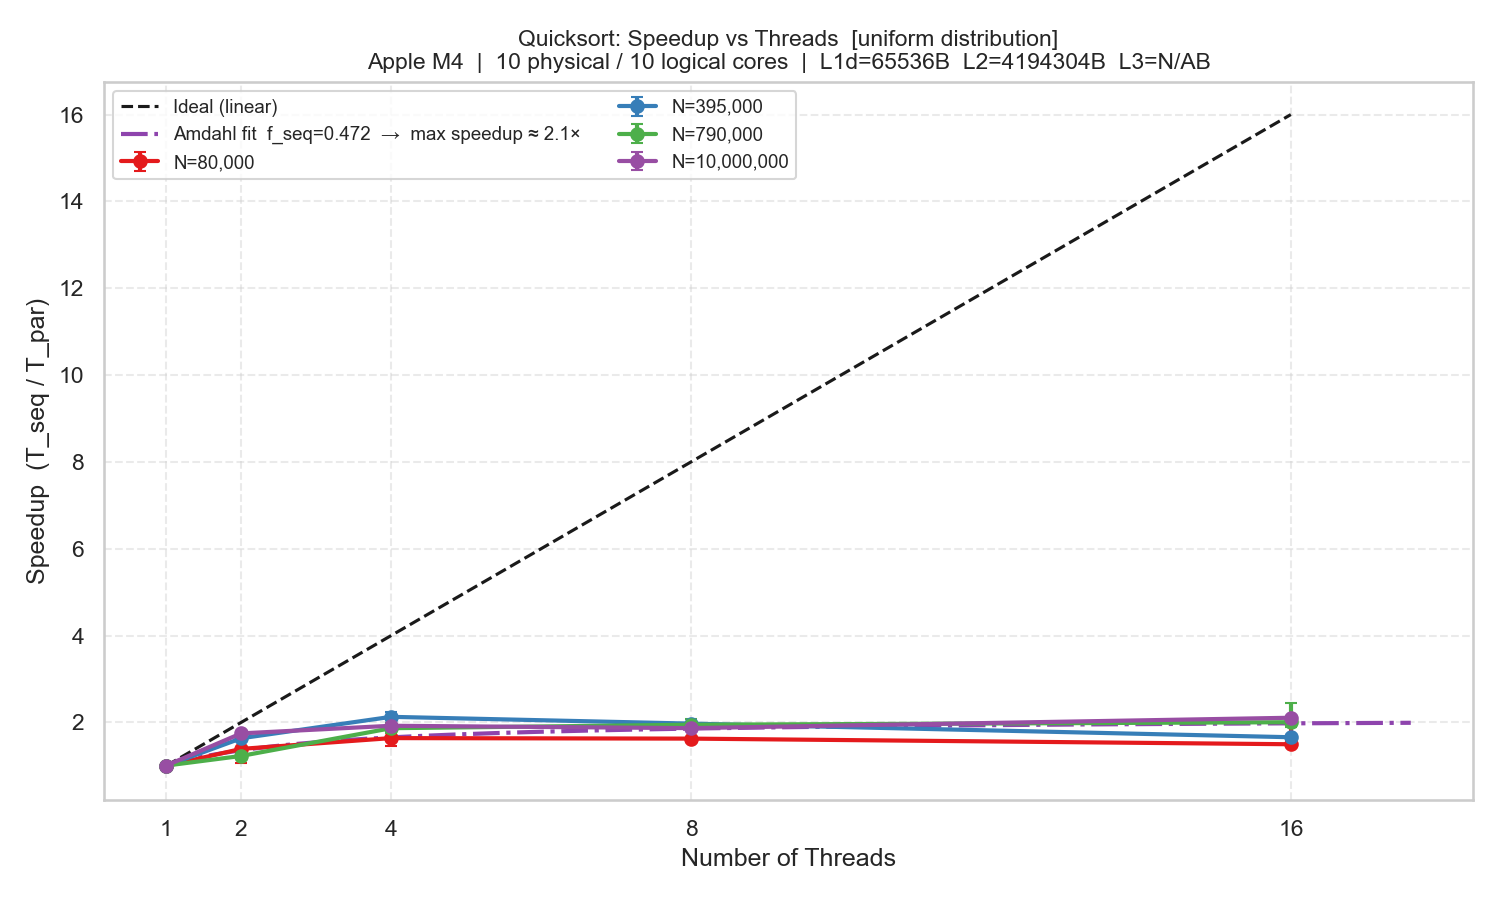
\includegraphics[width=0.48\textwidth]{../graphs/quicksort_speedup_vs_threads.png}
    \hfill
    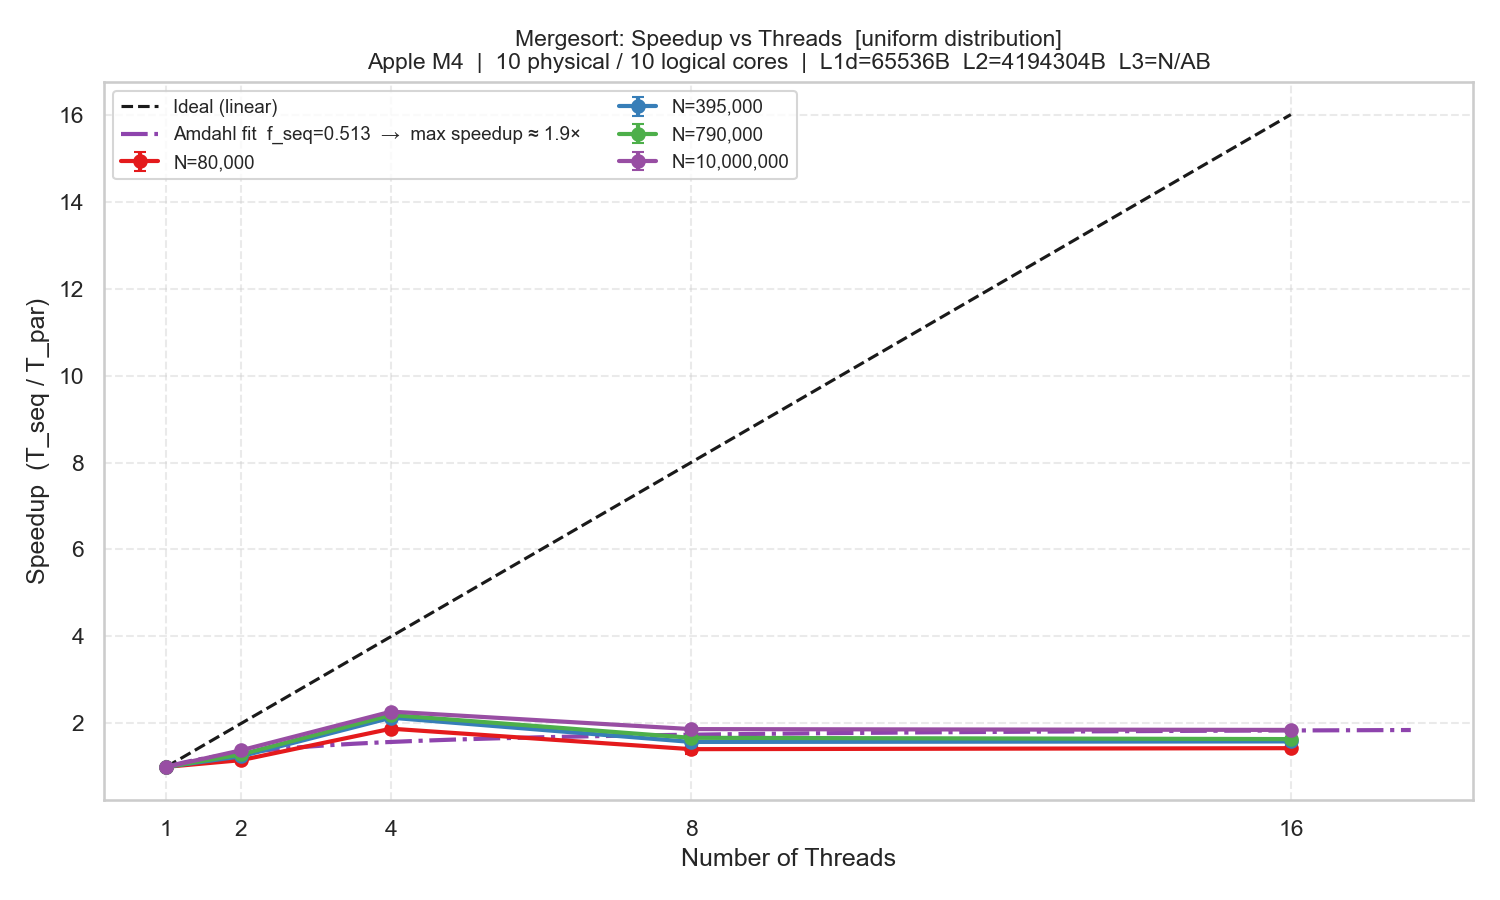
\includegraphics[width=0.48\textwidth]{../graphs/mergesort_speedup_vs_threads.png}
    \caption{Speedup vs Threads for Quicksort and Mergesort}
    \label{fig:speedup}
\end{figure}

When we plug our numbers into Amdahl's Law, we get:

\begin{center}
\begin{tabular}{lcc}
\toprule
Algorithm & Fitted $f_{\text{seq}}$ & Predicted max speedup \\
\midrule
Quicksort  & 0.481 & $\approx 2.1\times$ \\
Mergesort  & 0.518 & $\approx 1.9\times$ \\
\bottomrule
\end{tabular}
\end{center}

This indicates that approximately half of the computational work remains sequential, capping our maximum speedup at roughly $2\times$. The primary limiting factors are the unavoidable top-level merge and partition operations, combined with the initial overhead of thread creation and management.

\subsection{Efficiency}
Figure~\ref{fig:efficiency} demonstrates that parallel efficiency (defined as speedup divided by the number of threads) degrades rapidly as thread count increases.

\begin{figure}[htpb]
    \centering
    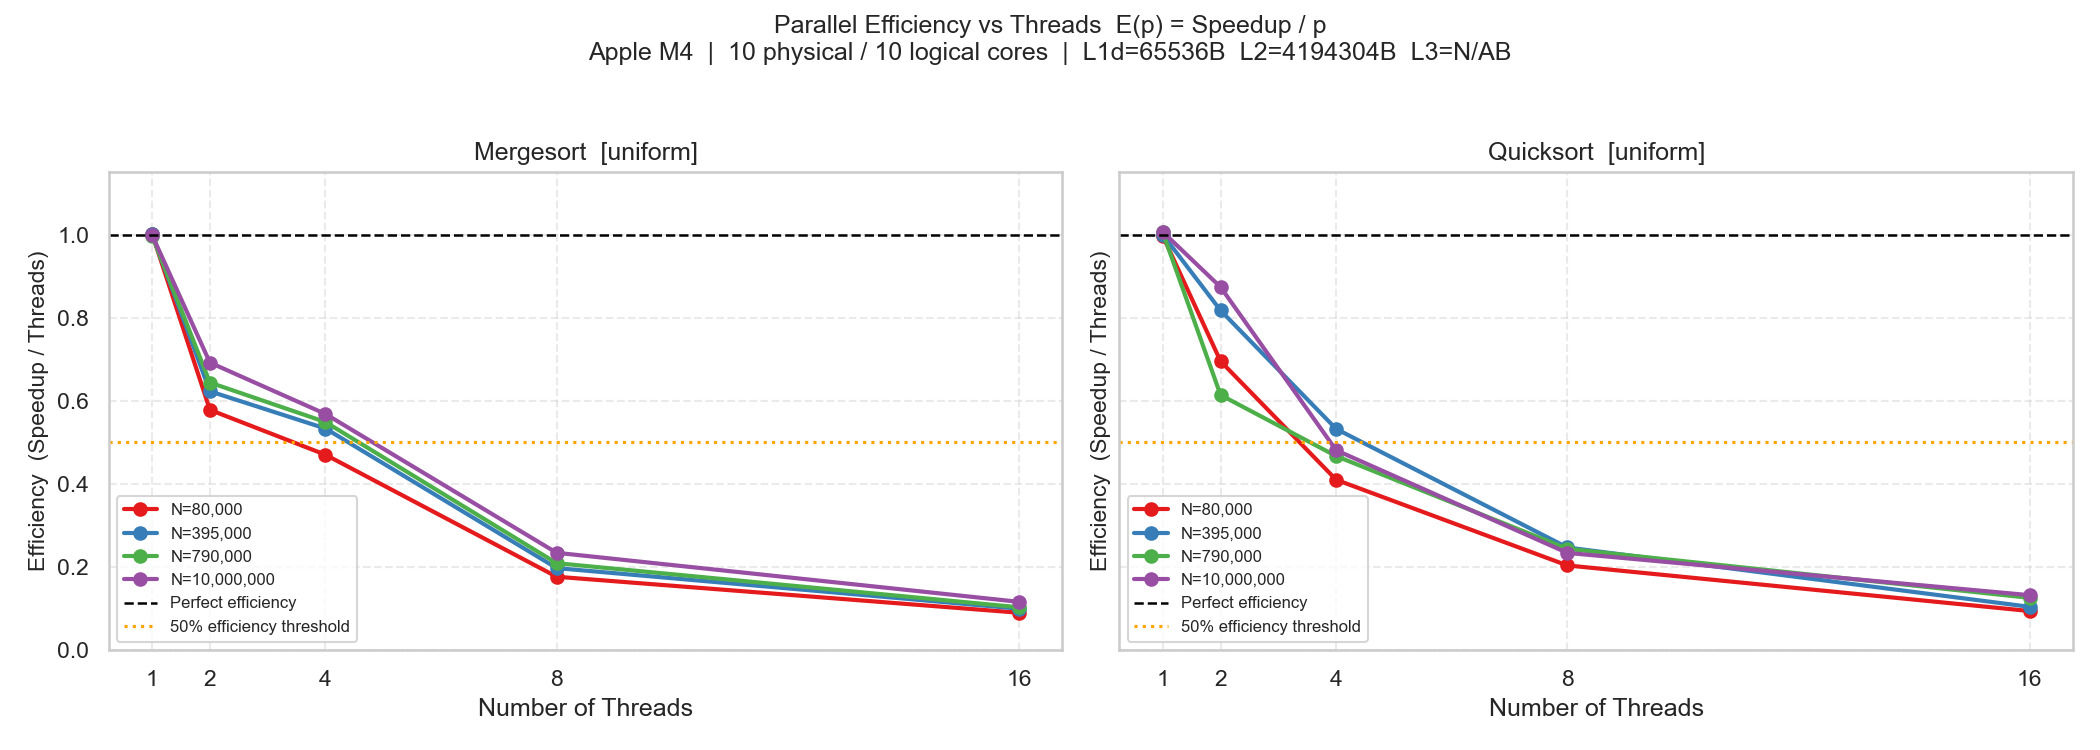
\includegraphics[width=0.8\textwidth]{../graphs/parallel_efficiency.png}
    \caption{Parallel Efficiency vs Threads}
    \label{fig:efficiency}
\end{figure}

It remains reasonable at 2 threads, but drops below 50\% by 8 threads. At 16 threads, which oversubscribes the available CPU cores, efficiency decreases sharply. Forcing the processor to manage an excessive number of threads introduces substantial context-switching overhead without yielding additional computational benefits.

\subsection{Effect of Distribution}
The input data distribution noticeably affects quicksort's performance, whereas its impact on mergesort is minimal. For arrays composed of identical elements, quicksort's three-way partitioning scheme resolves the array in $O(n)$ time, resulting in a major performance increase. Furthermore, for reverse-sorted data, the median-of-three pivot selection prevents the algorithm from degrading to $O(n^2)$ time complexity, maintaining the expected $O(n \log n)$ performance. In contrast, mergesort shows very stable execution times across all data distributions. As shown in Figure~\ref{fig:comparisons}, its comparison count closely tracks the theoretical $O(n \log n)$ curve regardless of the input distribution.

\begin{figure}[htpb]
    \centering
    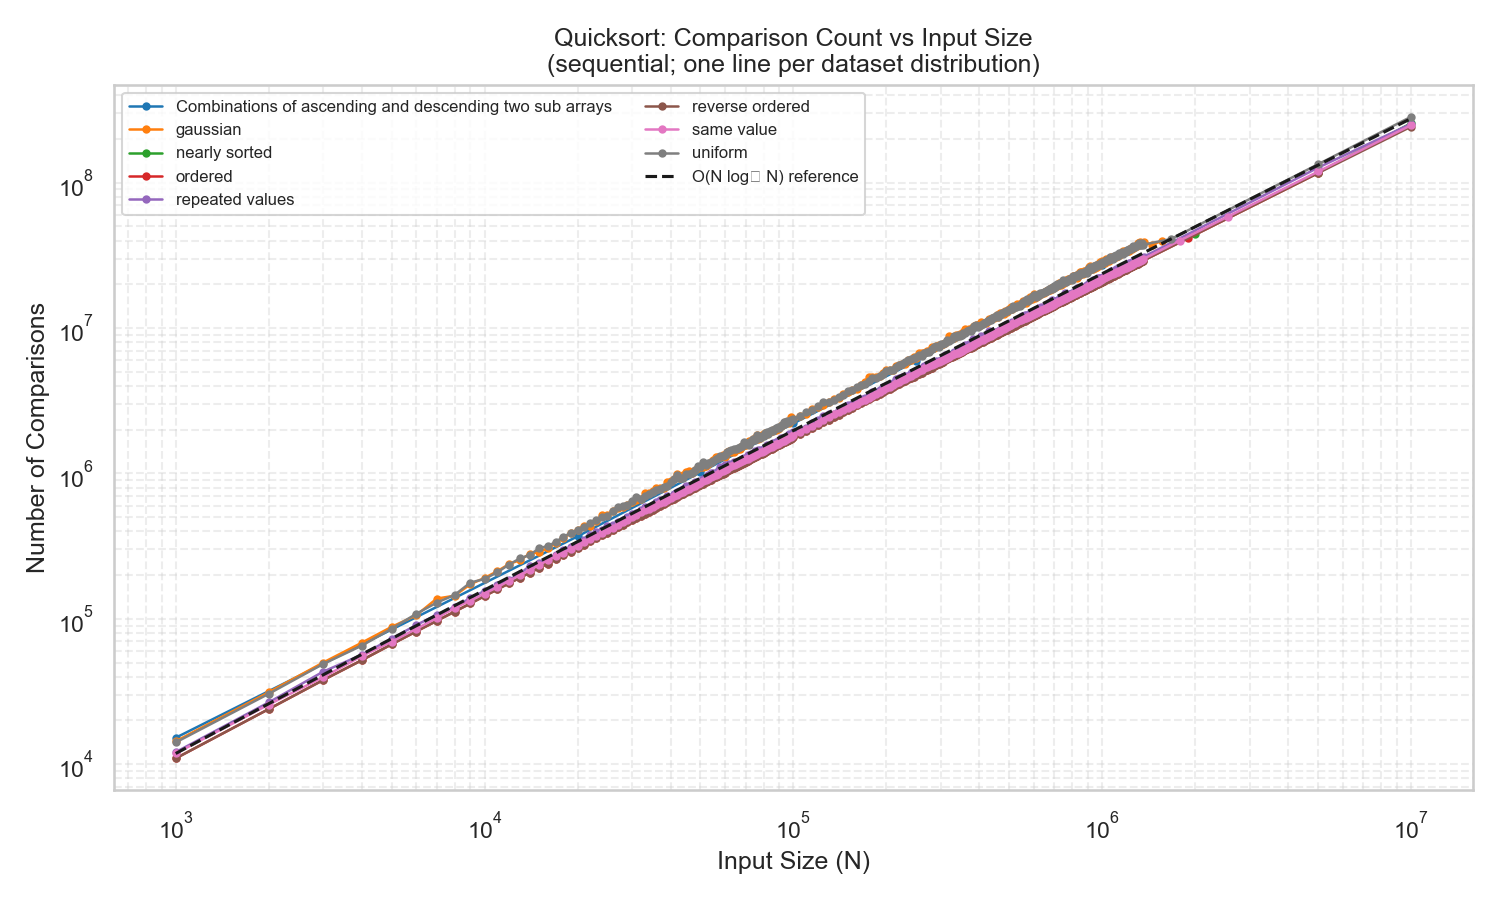
\includegraphics[width=0.49\textwidth]{../graphs/quicksort_comparisons_vs_size.png}
    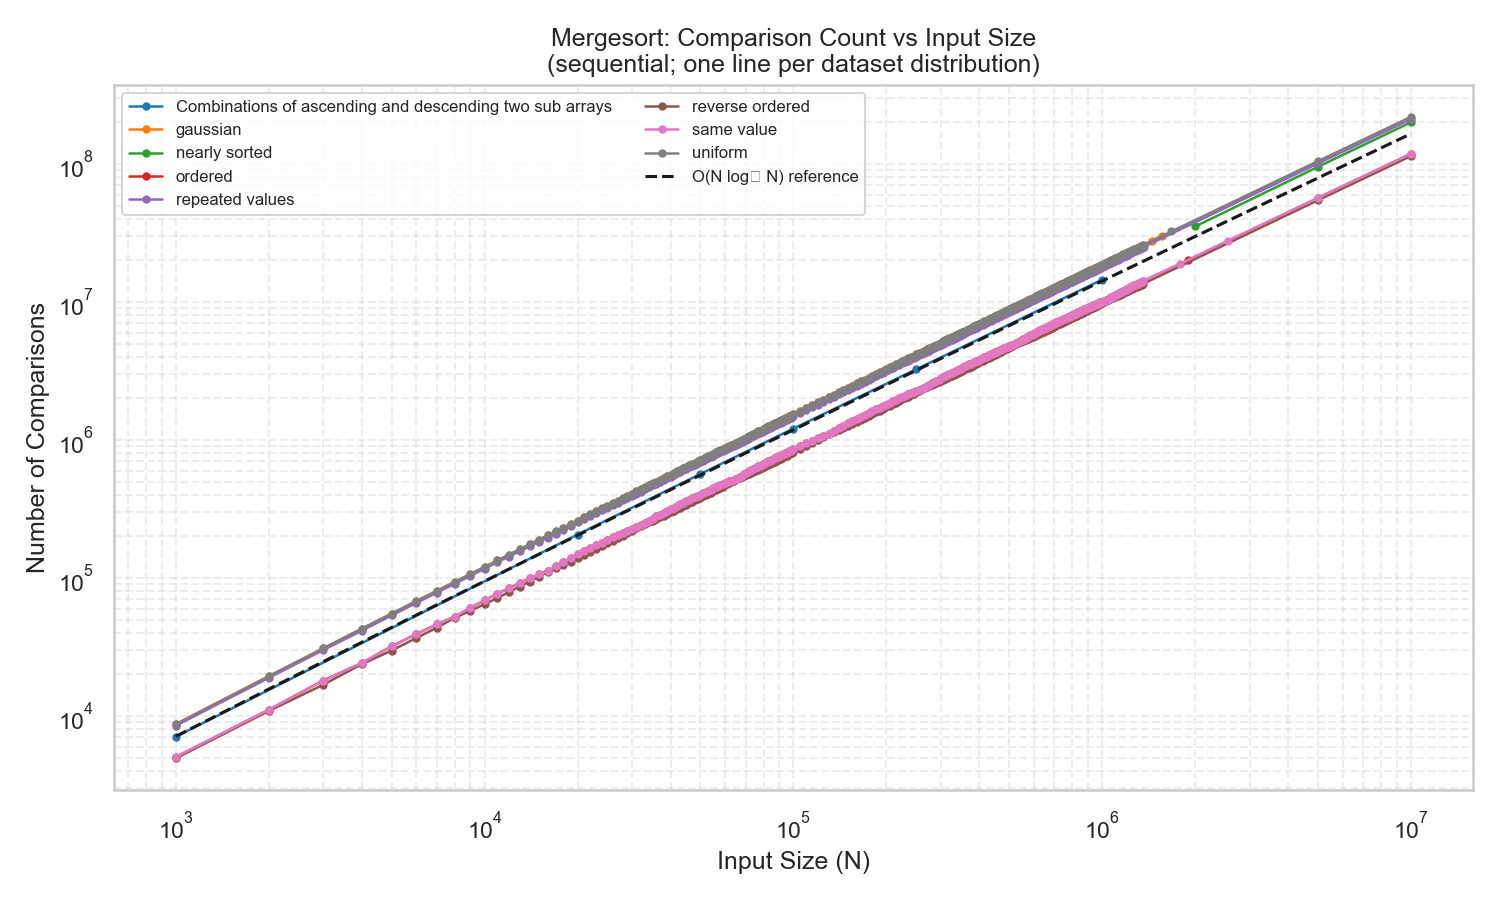
\includegraphics[width=0.49\textwidth]{../graphs/mergesort_comparisons_vs_size.png}
    \caption{Comparison count vs.\ input size for quicksort (left) and mergesort (right) across all six distributions, with $O(n \log n)$ reference.}
    \label{fig:comparisons}
\end{figure}

\subsection{Memory}
Mergesort requires an auxiliary buffer for its merge steps, meaning it uses more memory than quicksort, which sorts in place. Figure~\ref{fig:memory} shows that mergesort's peak memory usage is roughly double that of quicksort for all input sizes, and both scale linearly with $n$. This reflects a common trade-off: mergesort provides stable performance at the cost of higher memory consumption, whereas quicksort is more memory-efficient but its speed depends heavily on how the input data is distributed.

\begin{figure}[htpb]
    \centering
    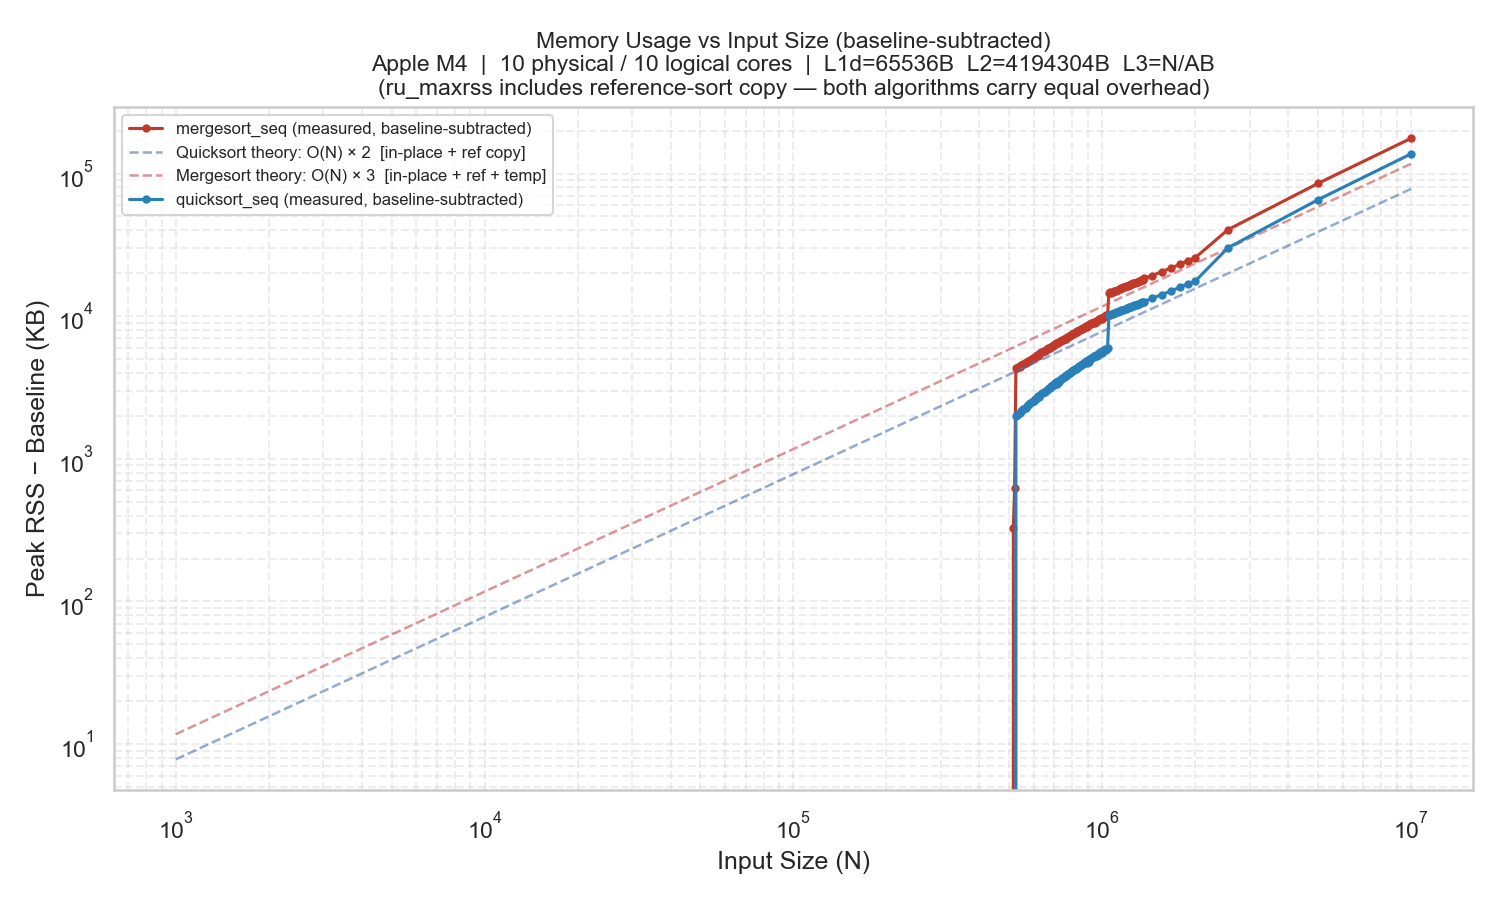
\includegraphics[width=0.8\textwidth]{../graphs/memory_comparison.png}
    \caption{Memory Usage Comparison vs Input Size}
    \label{fig:memory}
\end{figure}

\section{Discussion and Limitations}
Our results show that achieving large parallel speedups on these sorting algorithms is more difficult in practice than the theoretical model suggests. The sequential portions of both algorithms (the top-level merge in mergesort and the top-level partition in quicksort) place a hard ceiling on speedup that task-based parallelism alone cannot remove. Surpassing the observed 2x limit would require parallelizing these steps directly, which introduces extra complexity.

Additionally, here are some limitations of our approach worth noting:
\begin{itemize}
    \item The static thread-budget scheme does not adapt to load imbalance. When quicksort produces an uneven partition, threads assigned to the smaller subarray finish early and remain idle. A work-stealing scheduler like the one provided by OpenMP could mitigate this.
    \item Our experiments are limited to inputs of up to 10 million elements. At larger scales the fixed overhead of thread creation amortizes more favorably, and we would expect higher observed speedups.
    \item All measurements were collected on a single Apple M4 system. Results may vary on hardware with more cores.
\end{itemize}

\section{Team Plan and Contributions}
Akshat implemented the sequential and parallel quicksort algorithms. Aaron implemented the sequential and parallel mergesort algorithms. Aditya built the benchmarking pipeline, which included writing the benchmark driver and generating the performance visualizations. The team met regularly to discuss our implementations and share our progress. We then split the remaining reporting tasks evenly.

\begin{thebibliography}{9}
\bibitem{rosca}
Rosca, V.\ and C\u{a}rbureanu, M.
``A study on classic sorting algorithms.''
(Cited in our project proposal for the role of sorting in modern data-intensive
applications.)

\bibitem{kagglebench}
Akay, B.\ E.
``Benchmark Dataset for Sorting Algorithms.'' Kaggle.
\url{https://www.kaggle.com/datasets/bekiremirhanakay/benchmark-dataset-for-sorting-algorithms}

\bibitem{mergeparallel}
``Parallel Merge Sort.'' \emph{redixhumayun.github.io}, 2023.
\url{https://redixhumayun.github.io/systems/2023/12/29/parallel-merge-sort.html}

\bibitem{tsigas}
Tsigas, P.\ and Zhang, Y.
``A Simple, Fast Parallel Implementation of Quicksort and its Performance Evaluation on SUN Enterprise 10000.''
In \emph{Proceedings of the 11th Euromicro Conference on Parallel, Distributed and Network-Based Processing (PDP)}, 2003.
\url{https://www.cse.chalmers.se/~tsigas/papers/Pquick.pdf}

\bibitem{sciencedirect}
``A survey on parallel sorting algorithms on multicore processors.''
\emph{Future Generation Computer Systems}, Elsevier, 2024.
\url{https://www.sciencedirect.com/science/article/abs/pii/S0167739X24001225}

\bibitem{amdahl}
Amdahl, G.\ M.\ ``Validity of the single processor approach to achieving large scale
computing capabilities.'' AFIPS Conference Proceedings, 1967.

\end{thebibliography}

\end{document}